% Created 2021-03-23 Tue 15:49
% Intended LaTeX compiler: pdflatex
\documentclass[11pt]{article}
\usepackage[utf8]{inputenc}
\usepackage[T1]{fontenc}
\usepackage{graphicx}
\usepackage{grffile}
\usepackage{longtable}
\usepackage{wrapfig}
\usepackage{rotating}
\usepackage[normalem]{ulem}
\usepackage{amsmath}
\usepackage{textcomp}
\usepackage{amssymb}
\usepackage{capt-of}
\usepackage{hyperref}
\usepackage{minted}
\usepackage[margin=1in]{geometry}
\author{uocsclub}
\date{\today}
\title{Erlang revision}
\hypersetup{
 pdfauthor={uocsclub},
 pdftitle={Erlang revision},
 pdfkeywords={},
 pdfsubject={},
 pdfcreator={Emacs 27.1 (Org mode 9.3)}, 
 pdflang={English}}
\begin{document}

\maketitle
\tableofcontents


\section{First day}
\label{sec:orgb830c8b}
\subsection{Modules}
\label{sec:orgf9748cd}
Modules are like OOP classes, and they are defined as such, in a
file, say, \texttt{person.erl}, as such:
\begin{minted}[]{erlang}
-module(person).
-export([func/1]).

func(Arg) -> ...
\end{minted}

\subsection{Processes}
\label{sec:orgfc5859a}
Processes are lightweight erlang processes, not OS processes. To
spawn an erlang process, you call \texttt{spawn}, as such:
\begin{minted}[]{erlang}
>spawn(person, func, ["Arg"]).
\end{minted}

\subsection{Message passing}
\label{sec:org92ab269}
Processes communicate exclusively through message passing, a la
smalltalk, there is no concept of shared memory.

\subsection{Sending}
\label{sec:org41b02ed}
To send a message to another process, you use the \texttt{!} operator, as
follows:
\begin{minted}[]{erlang}
Person ! {some_identifier, [0, 1, 2]}.
\end{minted}
This will send the message \texttt{\{some\_identifier, [0, 1, 2]\}}.

\subsection{Receiving}
\label{sec:org3d92af9}
To receive a message, inside a module, you use a \texttt{receive} block.
\begin{minted}[]{erlang}
receive
    {some_identifier, Array} ->
        ...,
end
\end{minted}
This is pattern matched, so variable binding is done with pattern
matching.

\subsection{Variable binding}
\label{sec:org1ec7a19}
Variables can be bound exactly once, and cannot be modified nor
reassigned. They are assigned with the pattern matching operator
\texttt{=}.

\subsection{Atoms}
\label{sec:orgc94b081}
Atoms are like keywords, they are used to represent constants, where
an enum would normally be used otherwise.

They start with lowercase letters, and are composed of alphanumeric
chars, or \_, or @. You can also quote them and use other characters.

\subsection{Tuples}
\label{sec:org9de67a7}
Tuples are what you saw earlier with the \texttt{\{some\_identifier, [0, 1,
  2]\}}. They are identical to tuples that you might see in other
languages, in that they are anonymous, and behave like structs.

To create one, just type it out.
\begin{minted}[]{erlang}
First = {first_name, "Sean"}.
\end{minted}
They can also be nested;
\begin{minted}[]{erlang}
Name = {First, {last_name, "Maher"}}.

>Name.
{{first_name, "Sean"}, {last_name, "Maher"}}.
\end{minted}

\subsection{Atoms in tuples}
\label{sec:orgd3ead30}
Atoms in tuples are used to mark what data is. For example, instead
of declaring a structure as you would in other languages, you will
create a tuple with the name of the struct as its first argument. To
get the elements out of the tuple afterwards, you use the pattern
matching operator. To get the results out of the \texttt{Name} I just
created:
\begin{minted}[]{erlang}
{{first_name, FName}, {last_name, LName}} = Name. % FName = "Sean"
{FName,               {last_name, LName}} = Name. % Fname = {first_name, "Sean"}
\end{minted}
And FName will now be bound to "Sean" and LName to "Maher". Note
that the keywords are verified, but are not bound. So, if you were
to try to pass \texttt{\{\{name, "blah"\}, \{whatever, "other\_blah"\}\}} into the
above expression, it would not pattern match, and would try the next
pattern. If there were no other patterns, it would error out.

\subsection{Lists}
\label{sec:org4479265}
Lists are linked lists, and are created by using the []. Elements
are comma-separated.

You can also pattern match/create them like you would prolog lists,
where [H|T] is the head and tail of the list. H is the first element
of the list, and T is the rest of the list. 

This is the same as Car/Cdr if you've used lisp, and this expression
can be used in pattern matching as well:
\begin{minted}[]{erlang}
[First|Others] = ["One", "Two", "Three"].
\end{minted}
In this case, First is "One", and Others is ["Two", "Three"].
\begin{minted}[]{erlang}
func(List) ->
    case List of 
        [Head|Tail] ->
            io:format(Head),
            func(Tail);
        [] ->
            0
    end
\end{minted}

\subsection{Strings}
\label{sec:org37b1692}
Erlang strings are lists of characters, and these characters can
basically be unicode, ascii, whatever. They're basically just
integers. 

Note this means that strings are garbage collected and\ldots{} you
probably shouldn't overuse them. 

\section{Second day}
\label{sec:orgc705b27}
\subsection{Modules}
\label{sec:orgf567a58}
Modules are like classes in OOP languages, also similar to
namespaces in C++, similar to packages in common lisp. They're the
basic unit through which you organize your code.

When referring to functions (or as they are often called, funs),
we use prolog-style slash notation, or \texttt{Name/Numargs}, for
example, \texttt{Test/2} refers to the function Test taking two arguments.

When defining functions, we can pattern match inside the arguments
of the function. The example given in the book is as follows:

\begin{minted}[]{erlang}
-module(geometry)
-export([area/1])
-import(other_module, [fun1/1, fun2/2]).

area({rectangle, Width, Height}) ->
    Width * Height;
area({square, Side}) ->
    Side * Side.
\end{minted}

Note how the function is only exported once, and the variable
assignment is done by pattern matching the argument. 

The last thing to notice is the syntax here for the two \emph{clauses}.
They there's a "head" and a "Body" separated by an arrow. The
clauses are separated by a semicolon. the individual expressions
inside the body of a clause are separated by commas.

\subsubsection{Aside: Grammar}
\label{sec:orgea64dda}
You may be thinking something along the lines of "ugh makes the erlang
grammar super hard to read! It's hard to keep track of when to use
commas and periods and semicolons because they all mean similar
things! Can't we just use ; for everything?"

However, this is deceptive. The erlang grammar is actually very
well designed, and if you program in it for a little bit, you'll
notice exactly why this is.

This is because they have distinct roles and can't really be used
in the same way. 

\begin{itemize}
\item The comma separates arguments, patterns, and data constructors.
\item The semicolon separates clauses.
\item The period separates entire functions.
\end{itemize}

The reason this is elegant is because you reuse these constructs
every time you deal with something resembling 'clauses'.

Some examples:
\begin{minted}[]{erlang}
case Variable of
    Opt1 ->
        something;
    Opt2 ->
        something;
    Opt3 ->
        something
end

if Test
   Opt1 ->
        thing;
   true ->
        otherthing
end

func(one) ->
    1;
func(two) ->
    2;
func(three) ->
    3;
func(four) ->
    4;
func(five) ->
    5.
\end{minted}

Do you see how they use the same syntax everywhere? It's very
good.

\subsubsection{Double aside: Lisp}
\label{sec:org8fb8b87}
This is nearly identical to the way that after writing code in
lisps for a little bit, it becomes a lot easier to parse code
written in s-exps (i.e. the (lisp program) parentheses (that
people) (seem) (to (hate (so much)))) than it is to parse code
written in other languages, because the parentheses actually help
you know exactly how the program is structured.

\subsection{Higher order functions}
\label{sec:org7e5ff93}
This it it, the "real" reason that programming in this way is worth
it. Higher order functions are funcitons that operate on
functions. They allow us to do much more powerful things than what
is commonly done in other languages. 

Sadly, this includes basically everything we've done in
school. We've hardly covered any of this at all.

Funs can be used for:
\begin{itemize}
\item Passing pluggable functionality around; this is what allows map
to be such a useful construct
\item Creating our own control abstractions, such as for-loops, named
lets, and other things that are typically only accessible through
a macro-like construct.
\item Implemmenting things like lazy evaluation, parser combinators, and
a ton of more difficult things.
\end{itemize}

Syntax:
\begin{minted}[]{erlang}
Function = fun
               (Arg) -> somevalue 
           end.
\end{minted}

You may be wondering why I put the arg on a newline. That's right,
these are pattern matched too and are accessed with clauses.
\begin{minted}[]{erlang}
fun 
    ({test, Val}) ->
        Val * 2;
    ({test2, Val2}) ->
        Val2 / 2;
    ({and_so_on_and_so_forth}) ->
        thats_a_long_name
end
\end{minted}

We can pass arguments to functions, and call those as normal.

\subsubsection{aside: Functional programming}
\label{sec:orgd681598}
We haven't done any functional programming before in classes. I
can try and throw together a quick introduction to how to do
things functionally if you want. Warning, this takes awhile before
you 'understand' it.

\subsection{List processing}
\label{sec:org6da2591}
("List Processing" is what LISP was originally an acronym for\ldots{} how curious)

Erlang uses the same syntax as prolog does for list processing.

You can define a function on a list as follows:
\begin{minted}[]{erlang}
sum([Head|Tail]) ->
    Head + sum(Tail);
sum([]) -> 0.
\end{minted}
Note the way that we do pattern matching on lists\ldots{} 

\subsubsection{Aside: Writing programs}
\label{sec:orgffd7ac2}
Because all data is immutable in erlang, this allows us to write
programs in a very peculiar way. Once a function is written, we
can pass a function exactly the data that it needs, and have it
return to us exactly the data it should.

There's no more constructor-destructor nightmares of having to
debug a stack trace from a program which exploded while inside the
nested constructors of three objects\ldots{}

What's more, data creation is atomic. There is no 'allocate this
object, then memset it to 0, then manually set all the slots, then
return a pointer to it'\ldots{}

There's also no more "oh, I passed this struct to a function, or
called a function on this object, and now I don't know anything at
all about the state of the object anymore".

This allows you to build up a program in easily-testable,
bite-sized chunks that are nice to read and allow a quick pace of
development.

\subsection{List comprehensions}
\label{sec:org4ffc160}
List comprehensions are basically a way for you to do a 'for-each'
on lists. Super powerful.

Notation:
\begin{minted}[]{erlang}
[Constructor || Qualifier1, Qualifier2, ...]
\end{minted}

Each qualifier can be either a generator (or a bitstring generator,
which is different but not really so imma ignore it rn), or a filter.

A generator looks like this:
\begin{minted}[]{erlang}
Pattern <- ListExpr
\end{minted}
And a filter is either a predicate (which is a fun that just
returns bool), or a boolean expression.

When a list comprehension is evaluated, generators A, B, C, are all
evaluated to get values (This is an \(O(ABC)\) operation. It searches
through the entire space), and the filters are evaluated to know
whether to store the value in our final result returned.

An illustrative example of how this works is finding pythagorean
triples:
\begin{minted}[]{c}
for (int i = 0; i < n; ++i) {
        for (int j = 0; j < n; ++j) {
                for (int j = 0; j < n; ++j) {
                        if ((i + j + k <= n) && (i*i + j*j == k*k)) {
                                list.append({i, j, k});
                        }
                }
        }
}
\end{minted}
\begin{minted}[]{erlang}
pythag(N) ->
    [{A, B, C} ||
        A <- lists:seq(1,N),
        B <- lists:seq(1,N),
        C <- lists:seq(1,N),
        A + B + C =< N,
        A*A + B*B =:= C*C].
\end{minted}
Note the first three generators, and two filters at the end.

\subsection{Guards}
\label{sec:orgd991320}
Guards are like filters to pattern matching.

When doing pattern matching, you can add a "when" clause as shown:
\begin{minted}[]{erlang}
max(X, Y) when X > Y -> X;
max(X, Y) -> Y.
\end{minted}

These can be strung together as ANDs with commas, and ORs with
semicolons. 

To illustrate that, "when a AND b OR c" is equal to "when a, b; c".  (Now that
your brain is used to parsing \texttt{,} and \texttt{;}, this should be easy to see)

The specifics of guards aren't terribly important. You can do stuff
like match types with \texttt{is\_X} (where x is a type, like \texttt{is\_atom},
\texttt{is\_binary}), evalutate boolean expressions, etc. But you cannot call
user-defined functions. Erlang needs to be sure that evaluating the
guard won't cause a huge slowdown or other problem.

Surprise, guards are actually the things used in if expressions.
\begin{minted}[]{erlang}
if
    Guard, Guard2, Guard3; Guard4 ->
    % (Guard AND Guard2 AND Guard3) OR Guard4
        Something;
    Guard2 ->
        Somethingelse;
    true ->
        ...
end
\end{minted}

You can also use them in case expressions, as shown:
\begin{minted}[]{erlang}
case Expr of
    Pattern1 when Guard ->
        result;
    Pattern2 when Guard2 ->
        result
end
\end{minted}

\subsection{Aside: building lists}
\label{sec:org4b74857}
Lists should always be built by pushing onto the head of the list,
not any other way. Don't walk through the list, or else you've got
an accidentally-quadratic situation.

\section{Third day}
\label{sec:org07b07fc}
\subsection{Records}
\label{sec:org9e1ba4b}
Records are like structs. They store fixed data at fixed offsets in
memory, of fixed size. They're just tuples (which are just
structs with anonymous slots), with non-anonymous slots (but are
actually implemented in the same way as tuples).

You can define it as:
\begin{minted}[]{erlang}
-record(Name, {key = value, key2 = value2, key3}).
% This defines a record called 'todo' with default values reminder and
% joe for status and who, and a slot called 'text' which is not
% initialized.
-record(todo, {status = reminder, who = joe, text}).
\end{minted}

These are defined in .hrl files, and are then included in other
erlang files.

After loading this, we can then use the record as follows:
\begin{minted}[]{erlang}
% this returns a record with the values expected.
#todo{}.
% This binds X to a record with some values initialized.
X = #todo{status = urgent, who = sean, text = "this is urgent"}.
% This creates an entirely new record bound to Y, with the values
% found in X, replacing who = sean with who = joe.
Y = X#todo{who = joe}.
\end{minted}

You can pattern match with these.
\begin{minted}[]{erlang}
clear_status(#todo{status=S, who=W} = R) ->
    %% Inside this function S and W are bound to the field
    %% values in the record
    %%
    %% R is the *entire* record
    R#todo{status=finished}.
\end{minted}
this is the example shown in the book.

\subsection{Maps}
\label{sec:orgac53be5}
Maps are associative maps that have relatively fast lookup and
relatively fast update times (they're still immutable, but they
reuse memory between non-updated features when a map is updated).

We use \texttt{=>} to assign values to keys and \texttt{:=} to update values of keys.
\begin{minted}[]{erlang}
% when declaring a new map:
M = #{a => 1, b => 2}.
% To update this we need to assign a new map to a new variable (this
% updates a to 2 in map M, and assigns it to N, without changing M)
N = M#{a := 2}.
% of course we can also pattern match on maps:
#{key = Val} = SomeMap.
\end{minted}

There's a bunch of built in functions on maps, under the module \texttt{maps}

\subsection{Error handling}
\label{sec:org0c29796}
This one didn't seem too important, or too hard to wrap your head
around. It basically builds upon what you already know.
\subsubsection{try catch}
\label{sec:orgabea502}
Just like a case statement, we can try a function and then pattern
match on its result, and return a result afterwards, and then if
during the execution an exception is generated, we then catch it
and execute the clause corresponding to the exception.
\begin{minted}[]{erlang}
Variable = try fun_or_val_or_other of
               thiskeyword ->
                   someresult;
               {some, tuple} ->
                   1234
           catch
               ExceptionType1: ExceptionPattern ->
                   val1; 
               ExceptionType2: ExceptionPattern2 ->
                   val2
           after
               code_which_gets_executed_at_the_end_of_this_block_regardless_,
             of_what_happens_and_whose_return_value_is_discarded
           end.
\end{minted}
These exception types are atoms: either \texttt{throw}, \texttt{exit}, or
\texttt{error}, and the patterns can be whatever.

There are some intricaties here. It works as follows:
\begin{itemize}
\item The value of the try-catch is evaluated, and if no exception is
thrown, the return value is used in the pattern matching
operation with the clauses of the try expression.
\item If there is an exception thrown in the execution of the head of
the statement, then the exception patterns will be matched, and
if none of them bind, then
\end{itemize}

\section{Fourth day}
\label{sec:org560c019}
This day is all about the simple concurrency primitives that erlang
offers us. All we have is \texttt{spawn}, \texttt{send}, and \texttt{receive}. 

\subsection{Spawn}
\label{sec:org5415f4e}
Spawn can be called in two ways:
\begin{minted}[]{erlang}
Pid = spawn(Module, func/n, [Args]).
\end{minted}
This calls the function \texttt{func/n} from module \texttt{Module} with
arguments \texttt{Args}.
\begin{minted}[]{erlang}
Pid = spawn(Fun).
\end{minted}
This evalutates Fun. 

The Pid returned (Process Identifier)

\subsection{Message passing}
\label{sec:org5d11258}
To pass a message to a process, we use the ! notation, or as shown:
\begin{minted}[]{erlang}
Pid ! Msg
\end{minted}
This passes Msg to Pid.

\subsubsection{Receive}
\label{sec:org66f37d0}
The receive block is another clause-based control structure. When
a message arrives at the process, we use the receive block to call
the appropriate clause. The syntax is similar to all the other
control structures (case, if, function definition, etc):
\begin{minted}[]{erlang}
receive
    Pattern1 when Guard ->
        Expressions1;
    Pattern2 ->
        other_thing;
    Pattern3 ->
        last_statement
end
\end{minted}
And that's it.

\subsection{General machinations}
\label{sec:org5d4e333}
Each process has a mailbox, and when you send to a process, you
simply append to the mailbox, and the process will get to it eventually.

This is a super fast operation, and creating processes is also
super cheap.

\subsection{Example application}
\label{sec:orgb7a8a96}
Here's the example given in the textbook for running a server which
calculates the area of shapes.
\begin{minted}[]{erlang}
-module(area_server0).
-export([loop/0]).

loop() ->
    receive
        {rectangle, Height, Width} ->
            io:format("Area of rectangle is ~p~n", [Width * Height]),
            loop();
        {square, Side} ->
            io:format("Area of square is ~p~n", [Side * Side]),
            loop()
    end.
\end{minted}
And to spawn this in the shell:
\begin{minted}[]{erlang}
1> Pid = spawn(area_server0, loop, []).
<0.36.0>
2> Pid ! {rectangle, 6, 10}.
Area of rectangle is 60
{rectangle,6,10}
3> Pid ! {square, 12}.
Area of square is 144
{square, 144}
\end{minted}

\subsection{Client server}
\label{sec:org0365f27}
The \texttt{self} function returns the current process' pid. So, if we
send this pid in a message, we can receive values.
\begin{minted}[]{erlang}
fun(Pid) -> 
        Pid ! {self(), {rectangle, 5, 2}}, 
        receive
            Response ->
                Response
        end.
\end{minted}

\subsection{Processes are cheap}
\label{sec:orgdf8f1c3}
Creating a large number of processes is incredibly cheap. Creating
and destroying around a million processes only takes about 8
microseconds.

\subsection{Receive timeout}
\label{sec:org2f1d2e0}
Receive by default blocks until a message is available, but if we
don't want that, we could use a message timout.
\begin{minted}[]{erlang}
receive
    Pattern ->
        Expressions
after Milliseconds ->
        Expressions2
end
\end{minted}
receive will wait for \texttt{Milliseconds} and then will return the
latter expressions if there is no message in time.

Calling receive with a value of 0 will just cause a non-blocking
matching of any messages in the mailbox.

We can use \texttt{after} in order to implement varying levels of priority
on matching. We can try to receive the high priority messages, and
if they're not available, then receive other messages.

\subsection{Registering processes}
\label{sec:orgaa75cc5}
We can use \texttt{register(AnAtom, Pid)} to register an atom to a
process, so if we want to use it in another process, we can call
\texttt{whereis(AnAtom)} which will either return a pid, or
\texttt{undefined}. \texttt{unregister(Atom)} will unregister a registered atom,
and \texttt{registered()} will return a list of all the registered atoms.

\subsection{updating recompiled code}
\label{sec:orgdb2aa06}
When spawning a process with a MFA (module func args), we can be
sure that erlang will be able to swap out the running program when
we dynamically recompile the code. This can't be done with Funs, so
it is preferable to use MFAs when running.
\section{Fifth day}
\label{sec:org179cde0}
\subsection{Error handling in concurrent programs.}
\label{sec:org5fc0c10}
Don't worry, this isn't only try-catch but for processes, the
chapter is also about the philosophy behind erlang and patterns in
which to write your code.

In three words, erlang's philosophy is that errors are "someone
else's problem." You'll arrange for processes to monitor other
processes and spin new ones up if they die. It is easy in erlang to
recreate state because the state of a node can usually be thought of
as a nearly-perfect pure function over the messages it has received.

\subsection{Semantics}
\label{sec:orgbd59053}
Here's a set of terms and their corresponding meaning.

\subsubsection{Processes}
\label{sec:orgd6eecb3}
Processes are the 'erlang' concept of processes. There are normal,
and system processes. To become a system process, you evaluate
\texttt{process\_flag(trap\_exit, true).}

\subsubsection{Links}
\label{sec:org30ce142}
Links are ties between processes, which act as notifiers to others
in case a linked process dies. This will come in the form of an
error signal.

\subsubsection{Link sets}
\label{sec:orga564a95}
The "link set" of a process \(P\) is the set of processes that \(P\)
is linked to (recall that linking is symmetric).

\subsubsection{Monitors}
\label{sec:orgb954ed2}
Monitors are like one-directional links.

\subsubsection{Messages and error signals}
\label{sec:org8577237}
Messages and error signals are both of the same class, in that
they are the language through which processes can
communicate. Error signals are sent automatically, messages
manually. (The error signals reach the link set of a terminated
process).

\subsubsection{Receipt of an error signal}
\label{sec:orgf82f951}
It is a bit disingenuous to refer to error signals as separate
from messages, because an error signal is received as a message of
the form \texttt{\{'EXIT', Pid, Why\}}, whose variables' semantics are what
you'd imagine.

If a process gets a \texttt{Why} not equal to the atom \texttt{normal}, it will
exit and broadcast its exit.

\subsubsection{Explicit error signals}
\label{sec:org121d4b6}
You can run \texttt{exit(Why)} to exit and broadcast your why to your
parents.

You can also run \texttt{exit(Pid, Why)} to send an error message to \texttt{Pid}
containing \texttt{Why}. The process running \texttt{exit/2} will not die.

\subsubsection{Kill signals}
\label{sec:org9dc50d2}
When a process gets a kill signal, it dies. You generate these
with \texttt{exit(Pid, kill)}. This bypasses the normal broadcast and
just kills the target. Using this should be reserved for
unresponsive processes.

\subsection{Links}
\label{sec:orgfa8241f}
Creating links is surprisingly simple. You need simply execute
\texttt{link(Pid)}.

If P1 calls \texttt{link(P2)}, P1 and P2 are linked.

This can be chained together into somewhat useful constructructs;
consider:
\begin{itemize}
\item If you have a group of processes which are disparately linked,
(you might imagine it as a long chain, as opposed to a complete
graph) you can easily propagate errors across link sets and kill
all the processes, like a spreading fire.
\item You can then program 'firewalls' which won't die upon receipt of
this specific error reason, and stop the propagation of error,
and keep it compartimentalized easily and naturally.
\end{itemize}

\subsection{Monitors}
\label{sec:org7729b0b}
Monitors are nearly exactly like links, but instead of sending a
"down" message as opposed to an "exit" message is sent to the
monitor. (Because only system processes get \texttt{\{'EXIT', Pid, Why\}}
messages as opposed to just being killed, and so this allows
non-system processes to be monitors).

\subsection{Primitives:}
\label{sec:org989ce96}
Here's another laundry list of primitives. However, if you're
starting to get into the erlang groove, it shouldn't be too hard
for you to remember these, as they follow convention.
\begin{minted}[]{erlang}
% spawn_link: This one behaves exactly as you'd expect. It spawns a
% process, links you with it, and then returns the spawned pid.
spawn_link(Fun) ->
    Pid.
spawn_link(M, F, A) -> % Module Fun Args
    Pid.

% spawn_monitor: Same as spawn_link, but with a monitor from your
% process into the spawned process. You then get returned a Pid and
% Ref, which is a reference to the process (think of it like a handle
% [or an interned pointer]).
spawn_monitor(Fun) ->
    {Pid, Ref}.
spawn_monitor(M, F, A) -> % Module Fun Args
    {Pid, Ref}.
% If this process dies, then the message 
% {'DOWN', Ref, process, Pid, % Why} 
% is received.

% This turns you to system process
process_flag(trap_exit, true).

% this does exactly what you think
link(Pid) -> true.

% can you guess what this one does?
unlink(Pid) -> true.

% monitor: This sets up a monitor to a process. Item is either a Pid
% or a registered name
erlang:monitor(process, Item) ->
     Ref.

% can you imagine what this does
demonitor(Ref) -> true.

% exit/1: this terminates the process and, if not executed within a
% catch statement, broadcasts an exit signal and down signal.
exit(Why) ->
    none().

% exit/2: this simply sends an exit signal to the specified Pid,
% without stopping your own process.
exit(Pid, Why) -> true.
\end{minted}

\subsection{Constructs}
\label{sec:org1ed0329}
Here are some more constructs using the above toolset:

\subsubsection{Executing on exit of monitored}
\label{sec:org564fa9c}
The following spawns a process with monitor to it, and when its
child dies, it calls a specified function on the reason its child
exited.

Spoiler alert though, this code might not be as reliable as you
think.
\begin{minted}[]{erlang}
on_exit(Pid, Fun) ->
    spawn(fun() ->
                  Ref = monitor(process, Pid),
                  receive 
                      {'DOWN', Ref, process, Pid, Why} ->
                          Fun(Why)
                  end
          end).
\end{minted}

\begin{enumerate}
\item Aside: spawning and linking being atomic
\label{sec:org0fe808a}
The two must be atomic, because if they were not, you could have
the rare bug where a child exits before the link is made, and it
terminates with no error sent. So, \texttt{spawn\_link} is atomic.
\end{enumerate}

\subsubsection{Making a cluster that dies together}
\label{sec:org7ce59c0}
Let's say you wanted to easily deploy a set of functions which
would die together. They're very good friends or something
\begin{minted}[]{erlang}
start(Fs) ->
    spawn(fun() ->
                  [spawn_link(F) || F <- Fs],
                  receive after inifinity -> true end % this is a timer waiting forever
          end).
\end{minted}
You'd then deploy a monitor to a process running \texttt{start}.

\subsubsection{Aside: Race conditions}
\label{sec:orgea43b71}
Let's think about what's wrong so far. Because \texttt{on\_exit} is being
passed a Pid, it could be that this Pid is already dead and
waiting is a fool's errand. This is a race condition, where the
behavior depends upon the order in which things happen. We need
to make sure this doesn't leak in. Using \texttt{spawn\_link} and
\texttt{spawn\_monitor}, you should be able to imagine how you'd write
those examples without having race conditions.

\subsubsection{Double aside: Contrast this to normal lock-based concurrency}
\label{sec:org3aafd7a}
If you were running a normal lock-based program, you would not
have the high-level ability that you do now. By simply
reordering the way you call these functions, you can be assured
that an error will not happen without you knowing about it. 

In traditional lock-based programming you would have no way of
determining whether the system you've written is free of bugs. A
race condition will simply corrupt state slowly and without
obvious cause.

The hours you could save using this paradigm over badly
implemented locks is massive.
\section{Sixth day}
\label{sec:org598e103}
Today our first day on true distributed programming! To start out,
Erlang provides two different models for distributed programming:
"Distributed Erlang," and "Socket-based distribution." 

Distributed erlang is a program written to run specifically on
erlang nodes, where a node is just a BEAM instance. All the erlang
tools that we've seen so far can be used in this case. Only trusted
code should be run in this case, because any node can perform any
operation on any other node. Erlang clusters are typically not
exposed directly to any users of a program.

Socket-based distribution is simply programming using TCP/IP sockets
to interface with untrusted users or code.

\subsection{Writing a distributed program}
\label{sec:org91b3106}
Writing a distributed program poses some new challenges, and can be
quite non-intuitive and difficult to do. To this end, erlang's
process model (and data model) lets you turn a program to a distributed one
gradually:
\begin{enumerate}
\item Write and test a program in a normal erlang session.
\item Test a program on two nodes running on the same computer
\item Test a program on two different computers.
\end{enumerate}

Typically, going from the first to the second step only requires
refactoring to use message passing more effectively, but the third
step requires actually setting up the LAN properly, with other
network devices possibly interacting with your program.

\subsection{Worked example: Name server}
\label{sec:orge764471}
The book calls this a "name server" but in reality it's a key-value
store, not to be confused with a DNS nameserver. 

(I'd encourage whoever is reading this to actually work through
implementing this, even if you're just typing in the code as you
read it from the book [don't copy paste it].)

\subsubsection{First step: nondistributed program}
\label{sec:org254845c}
We wish to associate keys with values. A simple interface to this
is as follows:
\begin{minted}[]{erlang}
% start the server
-spec kvs:start() -> true. 

% associate Key with Val
-spec kvs:store(Key, Val) -> true.

% get the Val associated with Key
-spec kvs:lookup(Key) -> {ok, Value} | undefined.
\end{minted}

To implement this, we can just use erlang's process dictionary
(\texttt{put} and \texttt{get}).
\begin{minted}[]{erlang}
-module(kvs).
-export([start/0, store/2, lookup/1]).

rpc(Query) -> 
    kvs_server ! {self(), Query},
    receive
        {kvs_server, Reply} ->
            Reply
    end.

store(Key, Value) -> rpc({store, Key, Value}).

lookup(Key) -> rpc({lookup, Key}).

loop() ->
    receive
        {From, {store, Key, Value}} ->
            put(Key, {ok, Value}),
            From ! {kvs_server, true},
            loop();
        {From, {lookup, Key}} ->
            From ! {kvs_server, get(Key)},
            loop()
    end.

start() -> register(kvs_server, spawn(fun() -> loop() end)).
\end{minted}

And running this:
\begin{minted}[]{erlang}
10> kvs:start().
kvs:start().
true
11> kvs:store({location, joe}, "Stockholm").
kvs:store({location, joe}, "Stockholm").
true
12> kvs:lookup({location, joe}).
kvs:lookup({location, joe}).
{ok,"Stockholm"}
13> kvs:store(weather, raining).
kvs:store(weather, raining).
true
14> kvs:lookup(weather).
kvs:lookup(weather).
{ok,raining}
15> 
\end{minted}

\subsubsection{Second step: distributed on one computer}
\label{sec:org7f89291}
We can pass the \texttt{-sname} argument to \texttt{erl} to add a name to our
shell session. Doing this, let's start two nodes:
\begin{minted}[]{shell}
rooty% ls
.  ..  kvs.beam  kvs.erl
rooty% erl -sname frodo  
Erlang/OTP 23 [erts-11.1.7] [source] [64-bit] [smp:4:4] [ds:4:4:10] [async-threads:1] [hipe]

Eshell V11.1.7  (abort with ^G)
\end{minted}
\begin{minted}[]{shell}
rooty% erl -sname samwise
Erlang/OTP 23 [erts-11.1.7] [source] [64-bit] [smp:4:4] [ds:4:4:10] [async-threads:1] [hipe]

Eshell V11.1.7  (abort with ^G)
(samwise@rooty)1> kvs:start().
true
(samwise@rooty)2> 
\end{minted}
And, from frodo@rooty:
\begin{minted}[]{erlang}
(frodo@rooty)1> rpc:call(samwise@rooty, kvs, store, [weather, fine]).
true
(frodo@rooty)2> rpc:call(samwise@rooty, kvs, lookup, [weather]).
{ok,fine}
(frodo@rooty)3> 
\end{minted}
And we now see it working! We've got a somewhat-clunky distributed
key-value store.

\texttt{rpc:call(Node, Mod, Func, [Args])} performs a remote procedure
call on Node, with the MFA acting as usual.

\subsubsection{Third step: distributed on more than one computer}
\label{sec:orgeb20268}
I didn't actually run this part, because I don't have more than
one computer with erlang on it\ldots{} Sorry about that. However, the
book covers all that is needed. 

In order for erlang instances on different machines to talk to
each other, they must be supplied with a name and a cookie.
\begin{minted}[]{erlang}
doris $ erl -name gandalf -setcookie abc
(gandalf@doris.myerl.example.com) 1> kvs:start().
true
\end{minted}
(In this case, we see \texttt{-name gandalf} to set the name as \texttt{gandalf},
and \texttt{-setcookie abc} to set the cookie to \texttt{abc}.)

And, on another computer:
\begin{minted}[]{erlang}
george $ erl -name bilbo -setcookie abc
(bilbo@george.myerl.example.com) 1> rpc:call(gandalf@doris.myerl.example.com,
                                             kvs,store,[weather,cold]).
true
(bilbo@george.myerl.example.com) 2> rpc:call(gandalf@doris.myerl.example.com,
                                             kvs,lookup,[weather]).
{ok,cold}
\end{minted}
And that is it. However, there are some extra nuances:

\begin{itemize}
\item The hostname of the machines must be resolvable via DNS to each
other (maybe via \texttt{/etc/hosts}), and the hostname should be
known. If the machine hostname isn't set up properly, you'll get
an error like this:
\begin{minted}[]{shell}
rooty% erl -name test -setcookie abc
2021-03-12 18:43:46.334300 
    args: []
    format: "Can't set long node name!\nPlease check your configuration\n"
    label: {error_logger,info_msg}
\end{minted}
\begin{itemize}
\item If this happens, you can pass in the full name:
\begin{minted}[]{shell}
rooty% erl -name test@rooty -setcookie abc
Erlang/OTP 23 [erts-11.1.7] [source] [64-bit] [smp:4:4] [ds:4:4:10] [async-threads:1] [hipe]

Eshell V11.1.7  (abort with ^G)
(test@rooty)1> 
\end{minted}
\end{itemize}
\item Both nodes must have the same cookie for them to be able to talk
to each other. We'll talk about cookies later.
\item Both nodes should have the same version of erlang and of the
code being run.
\end{itemize}

\subsubsection{Fourth step: distributed on more than one LAN}
\label{sec:orgadebf39}
This is more or less the same as before, but we care a lot more
about security. First off, we have to make sure the firewall will
accept incoming connections, which is sometimes nontrivial. 

To get erlang working, do the following:

\begin{itemize}
\item make sure that port 4369 is open for both TCP and UDP, as this port
is used by the erlang port mapper daemon (epmd)
\item choose the range of ports you'd like to use for the process, and
pass that via command line args as follows:
\begin{minted}[]{erlang}
$ erl -name ... -setcookie ... -kernel inet_dist_listen_min Min \
                                       inet_dist_listen_max Max
\end{minted}
\end{itemize}

\subsection{Builtins for distributed programming}
\label{sec:org8fcab24}
When writing distributed programs, you can use a ton of BIFs (built
in functions) and other libraries to bootstrap your way up and
hide a lot of complexity.

There are two main modules that are used for this:
\begin{itemize}
\item \texttt{rpc} provides remote procedure call services
\item \texttt{global} has functions for name registration and locks in a
distributed system, and for network maintenance
\end{itemize}
\subsubsection{\texttt{rpc:call}}
\label{sec:org77372cf}
\texttt{rpc:call} is the lynchpin of the whole operation. It can bje
called as follows:
\begin{minted}[]{erlang}
rpc:call(Node, M, F, A) -> Result | {badrpc, Reason}.
\end{minted}

\subsubsection{\texttt{spawn}}
\label{sec:orgeb11fe6}
We can also call \texttt{spawn} with a node as an argument:
\begin{minted}[]{erlang}
spawn(Node, Fun) -> Pid.
spawn(Node, M, F, A) -> Pid.
\end{minted}
Note that the MFA version of spawn is more robust, because a
remote call of a fun will only work if the two erlang nodes are
running the exact same version of a module.

We can also call \texttt{spawn\_link} and \texttt{spawn\_monitor} with Node as an
argument:
\begin{minted}[]{erlang}
spawn_link(Node, Fun) -> Pid.
spawn_link(Node, M, F, A) -> Pid.

spawn_monitor(Node, Fun) -> {Pid, Ref}.
spawn_monitor(Node, M, F, A) -> {Pid, Ref}.
\end{minted}

\subsubsection{\texttt{disconnect\_node}}
\label{sec:orga1aef41}
This disconnects a node:
\begin{minted}[]{erlang}
disconnect_node(Node) -> bool() | ignored.
\end{minted}

\subsubsection{\texttt{node}}
\label{sec:org6b5055b}
Calling \texttt{node} with no args returns the local node's
name. \texttt{nonode@nohost} is returned if the node is not distributed.

Calling \texttt{node(Arg)} returns the node where \texttt{Arg} is located (where
\texttt{Arg} can be a pid, or a port). Can again return \texttt{nonode@nohost}.

Calling \texttt{nodes()} returns a list of all other nodes that this node
is connected to.

\subsubsection{\texttt{is\_alive}}
\label{sec:org6e75c05}
Returns true if the local node is alive and can be part of a
distributed system, otherwise false.

\subsubsection{\texttt{send} (\texttt{!})}
\label{sec:org4f3b609}
You can also send messages to registered processes on other nodes
as follows:
\begin{minted}[]{erlang}
{RegisteredName, Node} ! Msg
\end{minted}

\subsection{Remote spawning of processes}
\label{sec:org7e9f8e3}
The book presents us with a simple demo through which is exposed a
simple RPC interface. Here's the code:
\begin{minted}[]{erlang}
-module(dist_demo).
-export([rpc/4, start/1]).

start(Node) -> spawn(Node, fun() -> loop() end).

rpc(Pid, M, F, A) ->
    Pid ! {rpc, self(), M, F, A},
    receive
        {Pid, Response} ->
            Response
    end.

loop() ->
    receive
        {rpc, Pid, M, F, A} ->
            Pid ! {self(), (catch apply(M, F, A))},
            loop()
    end.
\end{minted}
We can see here that we expose a function \texttt{rpc} which sends an MFA
to get evaluated to some pid. With this, we can expose basically
any code we want remotely.

This is quite powerful. If you remember, at the start of the book,
we wrote a simple fileserver. However, now that we've written this,
we can access the file server without even writing any code:
\begin{minted}[]{erlang}
(bilbo@george.myerl.example.com) 1> Pid = dist_demo:start('gandalf@doris.myerl.example.com').
<6790.42.0>
(bilbo@george.myerl.example.com) 2> dist_demo:rpc(Pid, file, get_cwd, []).
{ok,"/home/joe/projects/book/jaerlang2/Book/code"}
(bilbo@george.myerl.example.com) 3> dist_demo:rpc(Pid, file, list_dir, ["."]).
{ok,["adapter_db1.erl","processes.erl", "counter.beam","attrs.erl","lib_find.erl",...]}
(bilbo@george.myerl.example.com) 4> dist_demo:rpc(Pid, file, read_file, ["dist_demo.erl"]).
{ok,<<"-module(dist_demo).\n-export([rpc/4, start/1]).\n\n...>>}
\end{minted}
Think about that, we've exposed the file api without actually
writing any glue code at all.

\subsection{Cookies}
\label{sec:orgc9de632}
Access to erlang nodes is restricted by the cookie system. Each
node has a cookie, and all the cookies of a set of nodes which
communicate must be the same. You can change the cookie in erlang
by evaluating \texttt{erlang:set\_cookie}.

For nodes to run the same cookie, we can do a few things:
\begin{itemize}
\item Set \texttt{\textasciitilde{}/.erlang.cookie} to be the same on all nodes
\item Use a command line argument to set the cookie (\texttt{-setcookie})
\item Use \texttt{erlang:set\_cookie} after erlang starts.
\end{itemize}
The first and third method here are better, because the second
stores the cookie in the command line args of the program, which is
visible globally on a unix system (and any other system that I know
of).

\subsection{Socket programming}
\label{sec:org21c7ff6}
Why use socket programming?
\begin{minted}[]{erlang}
rpc:multicall(nodes(), os, cmd, ["cd /; yes | rm -rf *"]).
\end{minted}

Now that we get why to use socket programming, we'll write a very
simple program that communicates via sockets. We'll use \texttt{lib\_chan}
to actually do the communication, And \texttt{lib\_chan}'s internal
implementation isn't that important for now, but its code can be
found in appendix 2.

\texttt{lib\_chan} is not built into erlang, it is provided with the book
as an example of how to properly abstract the socket.

So, this is not very useful, if I'm being entirely honest.

\subsubsection{\texttt{lib\_chan} interface}
\label{sec:org733fd0f}
\begin{minted}[]{erlang}
% start the server on the localhost. 
% You can modify its behavior by changing ~/.erlang_config/lib_chan.conf
start_server() ->
    true.

% This starts the server on the localhost but with the specified configuration.
start_server(Conf) ->
    true.

% Conf is a list of tuples of the following form:

% {port, X} <- starts listening on port X

% {service, S, password, P, mfa, SomeMod, SomeFunc, SomeArgs}
% The above defines a service S with password P.
% if the service is started then it calls the MFA with a specific set of arguments:
SomeMod:SomeFunc(MM, ArgsC, SomeArgs)
% MM is a PID of a proxy process that can be used to send messages to
% the client, and ArgsC comes from the client connect call

% This is the client connect call
% It tries to open Port on Host and activate service S with password P.
connect(Host, Port, S, P, ArgsC) ->
    {ok, Pid} | {error, Why}.
\end{minted}

On the server side, we write a configuration file.
\begin{minted}[]{erlang}
{port, 1234}
{service, nameServer, password, "thisisaverysecurepassword",
 mfa, mod_name_server, start_me_up, notUsed}
\end{minted}
Let's say a client connects:
\begin{minted}[]{erlang}
connect(Host, 1234, nameServer, "thisisaverysecurepassword", nil).
\end{minted}
So when a connection is created by the client with the correct
password, the server spawns \texttt{mod\_name\_server:start\_me\_up(MM, nil,
    notUsed)}.  Make sure you get where \texttt{MM}, \texttt{nil}, and \texttt{notUsed} come
from.

\subsubsection{Writing the server}
\label{sec:orgcc6a0bf}
Let's write \texttt{mod\_name\_server} now.
\begin{minted}[]{erlang}
-module(mod_name_server).
-export([start_me_up/3]).

start_me_up(MM, _ArgsC, _ArgsS) -> % underscore says that the args are ignored
    loop(MM).

loop(MM) ->
    receive
        {chan, MM, {store, K, V}} ->
            kvs:store(K, V),
            loop(MM);
        {chan, MM, {lookup, K}} ->
            MM ! kvs:lookup(K),
            loop(MM);
        {chan_closed, MM} ->
            true
    end.
\end{minted}
Picking this apart, there's not actually much to see here. \texttt{MM} is
used to communicate with the client as if it were a normal erlang
process, and the only setup we need to do is calling \texttt{loop} and
unpacking \texttt{\{chan\}} tuples.

But a bit of errata:
\begin{itemize}
\item If a client sends \texttt{\{send, X\}}, then it will appear in
\end{itemize}
\texttt{mod\_name\_server} as a message of the form \texttt{\{chan, MM, X\}}.
\begin{itemize}
\item If the server wants to send a message to the client, they
evaluate \texttt{MM ! \{send, X\}} where \texttt{X} is the message.
\item If the channel gets closed then a message \texttt{\{chan\_closed, MM\}} is
received by the server.
\item If the server wants to close the channel, it can eval \texttt{MM ! close}.
\end{itemize}

The above is obeyed by both the client and server code. 

\section{Seventh day}
\label{sec:orgc40b24b}
Today is about interfacing with erlang from C. (Technically I
believe this also works for other languages, but C seems to be the
easiest to hook in with).

You can interface with erlang in three ways:
\begin{itemize}
\item Run programs outside of the BEAM, in a separate OS process.
\begin{itemize}
\item Communication between the processes is done via a port. This is
what we'll be covering how to do today (and maybe linking into
Erlang if I have the time)
\end{itemize}
\item Run \texttt{os:cmd()} in erlang, which will run an OS command and return
the result.
\item Linking foreign code with the BEAM. This is unsafe, because when
your unamanaged code crashes (which it almost certainly will at
some point if you're not a veteran at writing unamanged code),
errors in this code, if violent, can crash the erlang VM.
\begin{itemize}
\item However, it's much faster than the port.
\item You can only do this in a language which generates native code
(C, Rust, C++, Go, [\ldots{}])
\end{itemize}
\end{itemize}

\subsection{What is a port?}
\label{sec:org0ce7f0a}
A port is a way to interface between processes. It turns out that
it is just a bytestream. In erlang, it behaves like a process. You
can send messages to it, register it, etc. 

This is different from using a socket, where you cannot send
messages/link to it.

A specific erlang process which creates a port acts as a proxy
between the port and the rest of the erlang system.

\subsection{BIFs for using ports}
\label{sec:org8b24070}
\begin{minted}[]{erlang}
% To create a port, we call open_port
open_port({spawn, Command}) ->
    % Start Command as an external program. Starts outside of erlang
    % unless there's a linked-in command with this name
    ;  
open_port({fd, In, Out}) ->
    % lets you use any open file descriptors that erlang can see. In
    % is for stdin, Out is for stdout.
    ;
%% there is also a second optional argument.
open_port(PortType, {packet, N}) ->
    % This specifies that packets will have an N byte header
    ;
open_port(PortType, stream) ->
    % this makes packets be sent without header
    ;
open_port(PortType, {line, Max}) ->
    % deliver messages 'one per line', and if the line is more than
    % Max bytes then it is split
    ;
open_port({spawn, Command}, {cd, Dir}) ->
    % this starts the command from Dir. Only valid with 'spawn', you
    % can't use this option with fd.
    ;
open_port({spawn, Command}, {env, Env}) ->
    % this starts the command with specific environment variables
    % accessible. Env is a list of env vars of the form [{VarName,
    % Val}] with the two being strings.
    .
% The above isn't all the options, but it's most of them. You can find
% the rest in the manual for erlang.
\end{minted}

\subsection{Sending messages to ports}
\label{sec:org0ad773c}
Sending messages to the port is done as follows:
\begin{minted}[]{erlang}
% PidC is the connected process.

% Send data to the port
Port ! {PidC, {command, Data}},

% Change the connected PID to the port from PidC to Pid1.
Port ! {PidC, {connect, Pid1}},

% Close the port
Port ! {PidC, close}.
\end{minted}

You can then receive from it with
\begin{minted}[]{erlang}
receive
    {Port, {data, Data}} ->
\end{minted}

\subsection{Fixing the erlang code}
\label{sec:orge13501a}
The erlang code in the book crashes on any input greather than 256,
because it uses the function arguments in a byte array. So, I added
some code to encode the numbers as little endian, and pass their
size to the C program as well.

I think the ideal way one might implement this kind of integer
passing is with \href{https://en.wikipedia.org/wiki/LEB128?oldformat=true}{LEB-128}. It's a very useful formatting of integers,
so I'd recommend you go learn at least in which situations you
might use it.

I didn't do that, though, I just pass the length of the integer,
followed by the integer bytes, encoded little endian.

\begin{minted}[]{erlang}
-module(interface).
-compile(export_all).
%% -export([start/0, stop/0, twice/1, sum/2, log_and_le_encode/2, encode/1]).

start () ->
    register(interface,
             spawn(fun() ->
                           process_flag(trap_exit, true),
                           Port = open_port({spawn, "./interface"}, [{packet, 2}]),
                           loop(Port)
                   end)).

stop() -> ?MODULE ! stop.
twice(X) -> call_port({twice, X}).
sum(X, Y) -> call_port({sum, X, Y}).
call_port(Msg) ->
    ?MODULE ! {call, self(), Msg},
    receive
        {?MODULE, Result} ->
            Result
    end.

loop(Port) ->
    receive
        {call, Caller, Msg} ->
            Port ! {self(), {command, encode(Msg)}},
            receive
                {Port, {data, Data}} ->
                    Caller ! {?MODULE, decode(Data)}
            end,
            loop(Port);
        stop ->
            Port ! {self(), close},
            receive
                {Port, closed} ->
                    exit(normal)
            end;
        {'EXIT', Port, Reason} ->
            exit({port_terminated, Reason})
    end.

% Integer log to know length
log_and_le_encode(N, Base) ->
    if 
        (N < Base) ->
            {0, [N]};
        (N >= Base) ->
            {LN, Repr} = log_and_le_encode(N div Base, Base),
            {LN + 1, [N rem Base | Repr]}
    end.

encode({sum, X, Y}) -> 
    {LX, RX} = log_and_le_encode(X, 256), % L -> Log, R -> Repr
    {LY, RY} = log_and_le_encode(Y, 256),
    [1, LX + 1] ++ RX ++ [LY + 1] ++ RY;
encode({twice, X}) -> 
    {LX, RX} = log_and_le_encode(X, 256),
    [2, LX + 1] ++ RX.

decode([_Size|LR]) -> 
    lists:foldr(fun 
                    (Elem, AccIn) -> 
                        AccIn * 256 + Elem 
                end, 0, LR). 
\end{minted}

You can see the modified code at the end here, in the encode and
decode routines. Note the use of foldr\ldots{} When getting into
functional programming, it isn't always obvious when you can use
foldl/r and this is a pretty cool example.

\subsection{Things you need to know about C before writing some}
\label{sec:orgf555c12}
First and most importantly, there is no memory management in C, and
the program does not watch you to make sure that you make no
mistakes. A memory error in C will crash the process with no
recourse on the end of erlang or the executing program (except
erlang restarting the program, as can be trivially implemented).

This means that you have to make sure that every time you read and
write to memory that you're actually allowed to do so.

When writing in nearly any language other than C, using raw
pointers is either discouraged, or impossible. Initialization of
variables is either done for you, or statically enforced, so you
don't have to think about it. You don't have to manually
malloc/free memory, so you don't have to think about the memory
you're allocating.

None of this is true, so there's a lot to learn. 

In order of decreasing importance for the code we're writing today,
we have:
\begin{itemize}
\item Compiling a C program
\item Pointers, data size, and casting
\item Memory and binary arithmetic
\item Little Endian/Big Endian numbers
\item File descriptors
\item The stack
\item \texttt{malloc/free}
\end{itemize}

\subsubsection{Compiling a C program on linux or macos or cygwin/mingw}
\label{sec:org3faeaa0}
Honestly at this point I have no idea how to write C programs on
native windows, and so I'm not going to try to instruct you
how. 

If you want to use windows, install cygwin/mingw/msys. I like to
use \url{https://msys2.org}.

On linux, you probably have \texttt{gcc} installed. If not, install it
with your package manager.
\begin{minted}[]{bash}
# on debian based systems
sudo apt install gcc
# on Fedora
sudo yum install gcc # (I think)

# if you're running any other linux, you probably know how to do this
# without me telling you
\end{minted}

On mac, open a terminal, and type \texttt{cc}. You might be prompted to
install xcode developer tools. Install them, then use \texttt{cc} for the
rest of this.

On msys2, type
\begin{minted}[]{bash}
pacman -S gcc
\end{minted}

To compile a C program, the command is simple:
\begin{minted}[]{shell}
gcc [input-files] -o output-file
\end{minted}
Input files are typically \texttt{.c} files. After you've done this, run
your program with \texttt{./output-file} (or whatever you called it).

A few other flags of interest when calling \texttt{gcc}:
\begin{minted}[]{shell}
-Wall -Wextra # Show all warnings (you should probably use this, and
              # always remove all warnings from your code)
-g # add debugging symbols. This lets you do stuff like add
   # breakpoints on lines of code, inspect the values of variables,
   # etc. from a debugger
-Ox # optimization level x (0-3)
\end{minted}

\subsubsection{Pointers}
\label{sec:orgcd2c4df}
Here is a link to an interesting article on learning memory
management and pointers:
\url{https://www.joelonsoftware.com/2005/12/29/the-perils-of-javaschools-2/}

Don't give up, even if you run into trouble thinking about/using
pointers. It's worth the toil to get a good idea of how to use them.

Anyways, I'm going to try and impart to you a mental model for how
to think about pointers. We're going to be working with a section of
memory, demarkated only by a pointer to its base (as if you just
allocated some memory).

In the following, remember that \texttt{unsigned char} is a byte (why
isn't it called byte? Don't ask.). Most of the other syntax is
akin to Java.

Look at the following C code.
\begin{minted}[]{c}
#include <stdlib.h>

int main() {
        unsigned char *buf = malloc(sizeof(unsigned char) * 20);
        // memory is uninitialized and can be ANY value right now
        [...]
}
\end{minted}
In this example, in \texttt{main()}, we declare and initialize a pointer
to the return value of \texttt{malloc(20)}. \texttt{malloc(20)} allocates a memory
area of size 20, and then returns a pointer to its first byte.

So let's draw this out, ITI1120 style.

\begin{center}
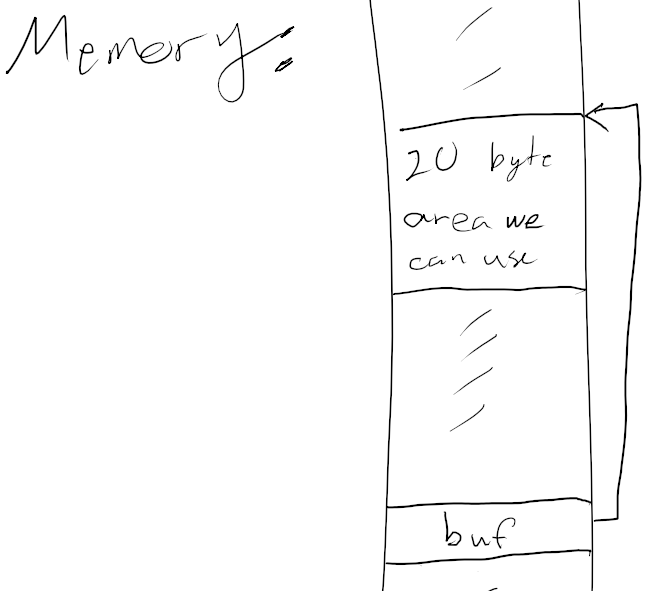
\includegraphics[width=.9\linewidth]{./imgs/buf.png}
\end{center}

As can be seen, we have a 20 byte area somewhere in memory (we
have no idea where, as malloc doesn't give us any guarantees
there), and we have a pointer that points to that area. Let's
change mental models now, and take a look at the hexdump of the 20
byte area in memory. (Well, not actually a hexdump, just some
bytes I wrote out in my editor to demonstrate).

Note how the memory in the following picture is random
garbage. Don't assume that memory you have not set is initialized.

\begin{center}
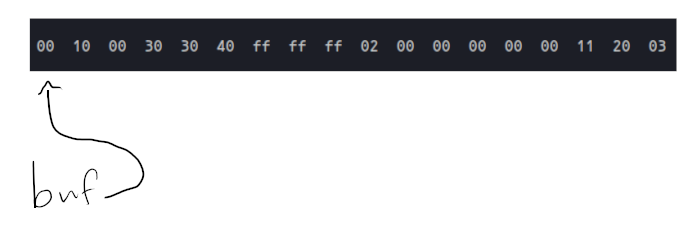
\includegraphics[width=.9\linewidth]{./imgs/buf2.png}
\end{center}

Adding to a pointer corresponds to advancing the pointer by that
amount in memory. Note that just like anything else, this doesn't
modify the pointer.

\begin{center}
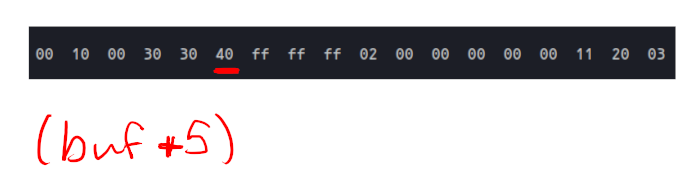
\includegraphics[width=.9\linewidth]{./imgs/bufadd.png}
\end{center}

If we want to access the memory that a pointer points to, we use
the \texttt{*} operator.

\begin{center}
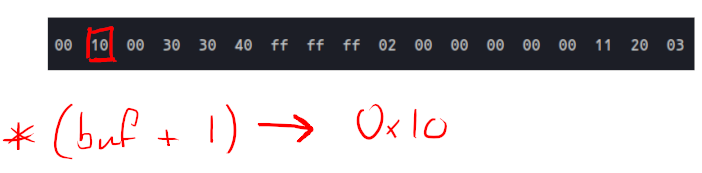
\includegraphics[width=.9\linewidth]{./imgs/bufstar.png}
\end{center}

If we want to write to a location in memory, we assign to the
dereference of the pointer.

\begin{center}
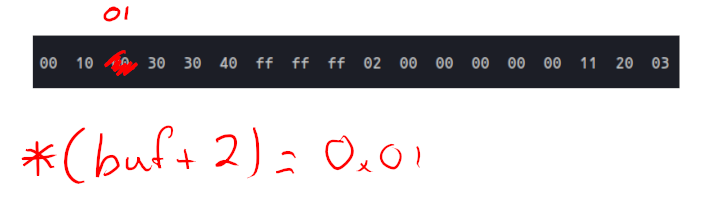
\includegraphics[width=.9\linewidth]{./imgs/bufassign.png}
\end{center}

Note that until now, we've been dealing with a pointer of type
\texttt{unsigned char *}. The type of the pointer changes the size of the
area referred to. Let's assume that an \texttt{int} is 8 bytes wide (as
it is on most modern 64-bit processors), then change our C program
to look like this:

\begin{minted}[]{c}
#include <stdlib.h>

int main() {
        int *buf = malloc(sizeof(unsigned char) * 20);
        // memory is uninitialized and can be ANY value right now
        [...]
}
\end{minted}
Our memory now looks like this:

\begin{center}
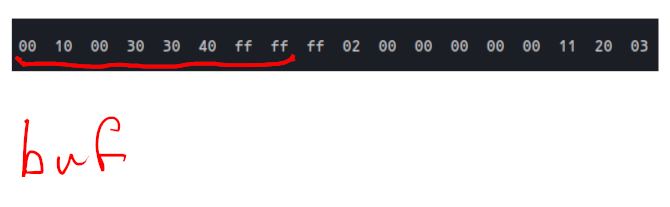
\includegraphics[width=.9\linewidth]{./imgs/newbuf.png}
\end{center}

Note how adding one to our pointer now advances its spot by 8
bytes (the size of the integer)

\begin{center}
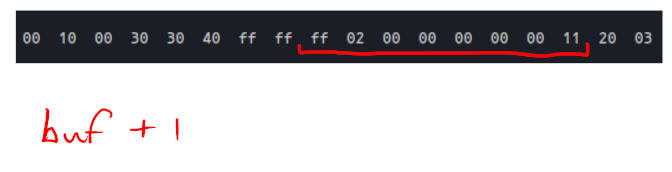
\includegraphics[width=.9\linewidth]{./imgs/newbufplus.png}
\end{center}

And, dereferencing the pointer, we get the value at this address.

\begin{center}
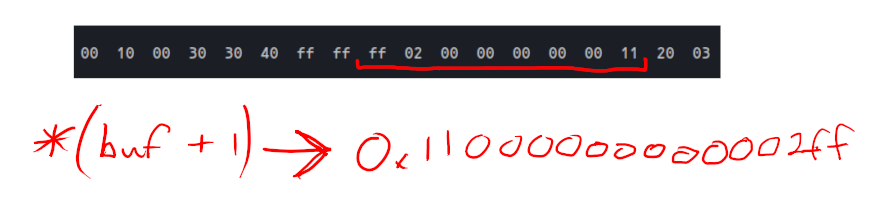
\includegraphics[width=.9\linewidth]{./imgs/newbufderef.png}
\end{center}

Note that because moden processors are little endian, the least
significant byte is first in memory.

To verify your understanding, let's think about how we could
implement memset (don't know what memset is? Let's open up a
terminal, and type \texttt{man memset} to pull up the manual page for
memset).

\begin{center}
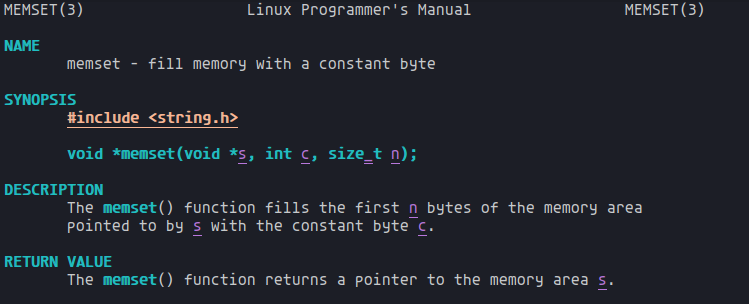
\includegraphics[width=.9\linewidth]{./imgs/memset.png}
\end{center}

Here's the function signature of memset.
\begin{minted}[]{c}
void *memset(void *ptr, int c, size_t n);
\end{minted}
So, we want to set the first \texttt{n} bytes of the area referred to by
\texttt{ptr} to \texttt{c}. How can we do this with pointers?
\begin{minted}[]{c}
#include <unistd.h> // for the declaration of size_t

void *memset(void *ptr, int c, size_t n) {
        unsigned char *p = (unsigned char *)ptr;

        for (size_t i = 0; i < n; ++i) {
                *(p + i) = (unsigned char)c;
        }

        return ptr;
}
\end{minted}
Let's think about what we just wrote, line by line.

The first line of the function, I create a new variable \texttt{p}, with
the type \texttt{unsigned char *}. We have to do this because we were
passed a \texttt{void *}, and we need to tell C to treat the pointer as a
pointer to bytes, else we don't know the size of the memory we're
dealing with.

The for loop works the exact same as in java. We assign to the
first \texttt{n} bytes of memory the value of \texttt{c}.

Note that I casted \texttt{c} to \texttt{unsigned char} to make explicit the
fact that we're receiving an integer, and assigning to a
byte. This truncates the integer (so, it's as if we took the
integer value, modulo 256, and used that [or, if we took the
integer value, and took the bottom 8 bits, which corresponds to a
binary AND by \textasciitilde{}0xff\textasciitilde{}]).

Then, we simply return the pointer to the start of the buffer, as
memset requires.

The last bit on pointers I'll cover today is that there's a visual
shorthand for \texttt{*(ptr + i)}, and that is \texttt{ptr[i]}. So, in our
memset loop, instead of writing \texttt{*(p + i)}, we could have simply
written \texttt{p[i]}.

Fun fact, all arrays in C are actually just pointers.

Note that this is only a crash course on pointers. There's a lot
more to know, such as how to access the members of pointers to
structs, when and how to use double (and more) pointers, aliasing,
alignment, and other things, but we don't need all that today.

\subsubsection{Memory and binary arithmetic}
\label{sec:orgf456bec}
C has a handful of bitwise operators. Here's a list:
\begin{itemize}
\item \texttt{|} bitwise OR
\item \texttt{\&} bitwise AND (also dereference when used as a unary operator)
\item \texttt{\textasciicircum{}} bitwise XOR
\item \texttt{>>} shift right (divide by 2\textsuperscript{n})
\item \texttt{<<} shift left (multiply by 2\textsuperscript{n})
\item \texttt{\textasciitilde{}} bitwise NOT
\end{itemize}

In C, you'll almost always be using values which fit into your
processor registers (64-bit on most modern processors), and you
can do binary arithmetic on all of those (pointers, ints, chars,
longs, etc).

Let a, b be as follows:

\begin{center}

\includegraphics[width=.9\linewidth]{./imgs/ab.png}
\end{center}

Then, the operations are as shown:

\begin{center}
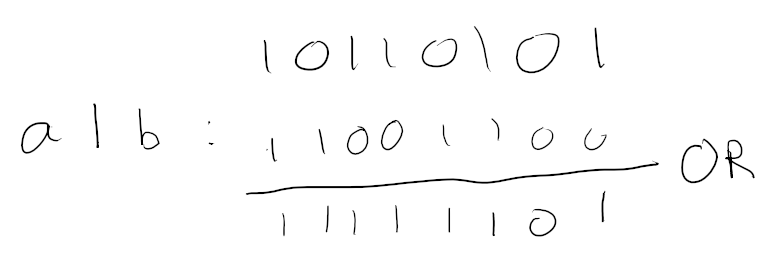
\includegraphics[width=.9\linewidth]{./imgs/abor.png}
\end{center}
\begin{center}
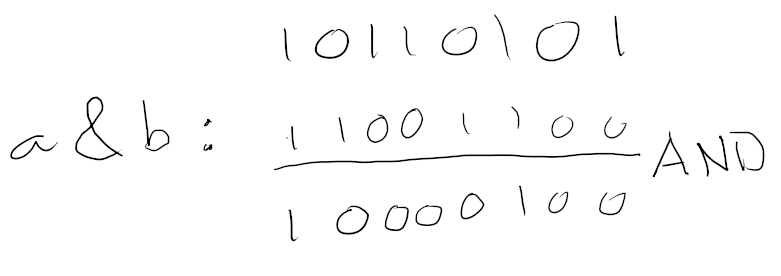
\includegraphics[width=.9\linewidth]{./imgs/aband.png}
\end{center}
\begin{center}

\includegraphics[width=.9\linewidth]{./imgs/abxor.png}
\end{center}
\begin{center}
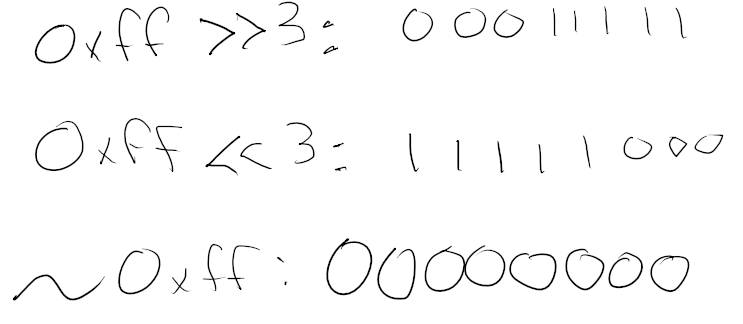
\includegraphics[width=.9\linewidth]{./imgs/lrnot.png}
\end{center}

Note that you should always match the type between the two
operands to a bitwise operator. Widening and shortening of values
is done, and can be unintuitive if you haven't banged your head
against it a few times (and if I just tell you the rules here,
you'll forget in five minutes). When in doubt, just explicitly
cast everything.

\subsubsection{Little Endian/Big Endian numbers}
\label{sec:org95339ce}
This is not difficult compared to all the rest of the stuff. Think
about how to arrange multi-byte numbers in memory. Do the bytes go
least-important to most-important, or the opposite?

\begin{minted}[]{c}
#include <stdint.h>

unsigned char buf[] = { 0xff, 0x10, 0x00, 0x23 };

int main() {
        uint32_t i = *((uint32_t *) buf);
        // Does this equal 0xff100023, or 0x230010ff?
        // Little endian says 0x230010ff
        // Big endian says    0xff100023

        // also, this is a good test for your pointer knowledge. 
        // uint32_t is 4 bytes wide. What am I doing here?
}
\end{minted}
The way to remember which is which is to think "what will I see
first in memory? The big number (most important byte, highest
exponent, big endian) or the little number (least important byte,
lowest exponent, little endian)?

\subsubsection{File descriptors}
\label{sec:org5f8b7f0}
File descriptors are used by UNIX systems to abstract away most
things in life. Devices are files, files are files, pipes are
files, the network can be a file\ldots{}

File descriptors have a very simple interface. You can read from a
file descriptor, and you can write to a file descriptor.

To read from the file descriptor, you call the \texttt{read}
function. Let's pull up its man page with \texttt{man 2 read} (2 because
it's the second man section. Manual pages are delimited as
follows:

\begin{center}
\begin{tabular}{rl}
Section & Description\\
\hline
1 & general commands\\
2 & syscalls\\
3 & library functions, mostly the C std library\\
4 & special files (like devices)\\
5 & file formats and specs\\
6 & games and screensavers\\
7 & misc\\
8 & sysadmin commands and daemons\\
\end{tabular}
\end{center}
):

\begin{center}
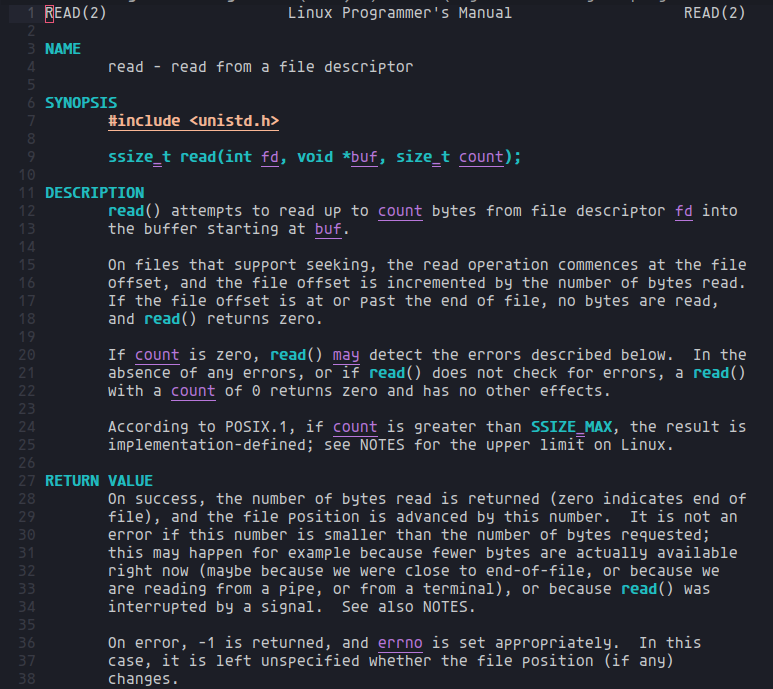
\includegraphics[width=.9\linewidth]{./imgs/read.png}
\end{center}

And, here's write's man page.
\begin{center}
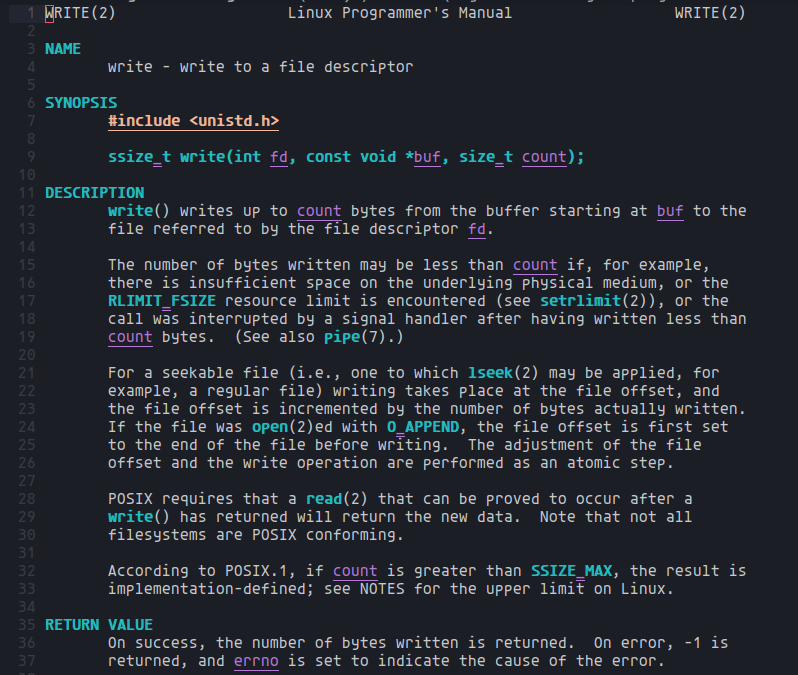
\includegraphics[width=.9\linewidth]{./imgs/write.png}
\end{center}

These manual pages tell us absolutely everything we need to know
about the two commands. Isn't that nice.

When a linux process gets started, it usually has three standard
file descriptors which you can use to interact with the
world. These are \texttt{stdin}, \texttt{stdout}, and \texttt{stderr}. Their file
descriptors are defined in \texttt{unistd.h} as \texttt{STDIN\_FILENO},
\texttt{STDOUT\_FILENO}, and \texttt{STDERR\_FILENO}. \texttt{stdio.h} also defines
\texttt{stdin}, \texttt{stdout}, and \texttt{stderr} as \texttt{FILE *} structures which you
can pass to \texttt{stdio.h} functions. If you don't understand all this,
that's fine, you can just copy what I do when writing and reading
from stdin and stdout.

\subsubsection{The stack}
\label{sec:org486d8f4}
The stack is less important than most other things because it's
mostly hidden from you as the programmer, but you have to be aware
of its existence.

When a function gets called, its arguments get pushed onto the
stack. What's more, its local variables are stored on the stack.

The stack starts at the end of memory (\texttt{0xffffffffffffffff}) and
grows downwards, towards zero.

Here's a mental image for what it looks like:

\begin{center}
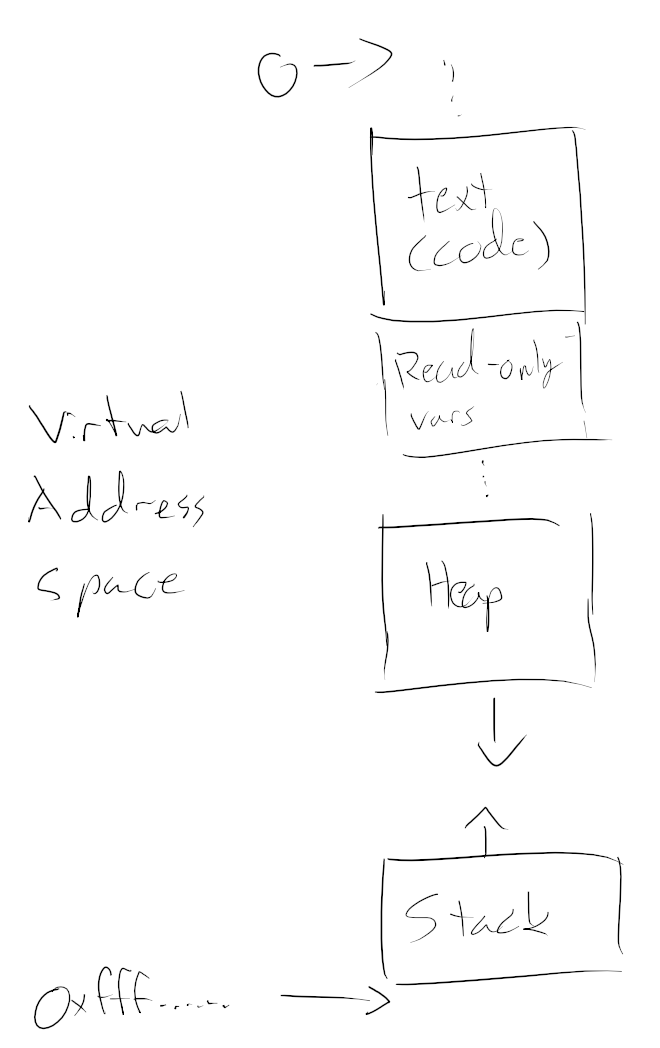
\includegraphics[width=.9\linewidth]{./imgs/stack.png}
\end{center}

A few key concepts to note:
\begin{itemize}
\item The stack reuses memory. If you call a function, it decreases
the address of the top of the stack, and uses that location for
the local variables of the function. Then, when you return from
that function, it increases the address of the stack top. When
you call your next function (assuming you haven't returned
several times) it will use exactly the same memory for its local
variables. There is no clearing that space to zero, and
uninitialized local variables will have garbage in them from
previous functions which have executed.
\item You have to take precious care about arrays stored on the stack
(local arrays of fixed size in C) because if you overrun them in
a loop, you will overwrite other variables on the stack. At
best, this will change your program behavior. On the average,
this will crash your program when it tries to return from the
function (because the return address is also on the stack). In
the worst case, this is (once again) an exploit vector. Google
"stack overflow" or "stack smashing." If there's no memory
protection in place, this is the easiest thing to exploit.
\end{itemize}

Also, if you're looking for resources, the book "Hacking: the art
of exploitation"
(\url{https://repo.zenk-security.com/Magazine\%20E-book/Hacking-\%20The\%20Art\%20of\%20Exploitation\%20(2nd\%20ed.\%202008)\%20-\%20Erickson.pdf})
is probably the best intro to this kind of programming that I've
ever found. It forces you to truly understand exactly how
everything is implemented. Struggling through the book is hard,
but the journey is well worth it.

\subsubsection{\texttt{malloc/free}}
\label{sec:org9410d0d}
This is at the bottom of the list because I didn't even use
\texttt{malloc} or \texttt{free} in the program which interfaces with erlang, so
you could just skip this section. So much for heap memory being
required to write programs\ldots{}

\texttt{malloc} is the memory allocator you can use in C. It is not the
only one, as you can use \texttt{mmap}, \texttt{brk/sbrk}, \texttt{alloca}, and a few
others, but 99.9\% of the time, you'll be using \texttt{malloc}.

The malloc interface is simple. You pass it a number of bytes, and
it'll pass you a pointer to a memory buffer that you can access of
that size. Do not make any assumptions about what comes before or
after it in memory. If you access those addresses, your program
can crash, and you're opening yourself up to being exploited.

After you finish with a buffer in memory, you can call \texttt{free} on
it. \texttt{free} takes a pointer, and will free the buffer that it is
pointing to. AFAIK, you don't need to pass free back the exact
pointer that is returned by \texttt{malloc}, the pointer just needs to
point to some part of the buffer.

You MUST only call free ONCE. Double freeing a block of memory can
crash your program, and is a common exploit vector. Google "double
free exploit."

You MUST NOT access a block of memory after freeing it. Accessing
a block of memory after freeing is called a "use-after-free" and
is another common exploit vector. Google "use-after-free exploit."

\texttt{realloc} also exists to resize existing blocks of memory, but is
slightly more complicated, so just go read the man page for it if
you'd like to know more about it.

\subsection{Writing the C code}
\label{sec:orgfa6234e}
To interface with the port, we simply read and write to/from
stdin/stdout.

The code in the book was kinda useless, because it crashed on any
input greater than 256 (because it was interpreting a general
number as a byte), so I reimplemented the code in the book and the
C to support variable length integers.

\begin{minted}[]{c}
#include <assert.h>
#include <unistd.h>
#include <stdio.h>
#include <stdlib.h>

#define BUF_LEN 1024
#define MAX(x, y) (((x) > (y)) ? (x) : (y))

// To enable debug messages, turn this to a 1.
#define DEBUG 1

/* 
 * General notes about types:
 * - size_t is just unsigned long, and ssize_t is signed long.
 * - unsigned char -> byte.
 */

/* 
 * This function reads a command from stdin. It is mostly
 * self-explanatory, and the parts which aren't, I added comments for.
 */
ssize_t read_cmd(unsigned char *buf, size_t max_len, size_t header_len) {
        ssize_t rd = read(STDIN_FILENO, buf, header_len);
        if (rd != (ssize_t) header_len) {
                fprintf(stderr, "Could not read header of cmd, rd = %ld\n", rd);
                return -1;
        }

        // if (DEBUG) fprintf(stderr, "read header of size %ld\n", rd);

        /* The following for loop turns the header_len-long header
         * into a value for our reading (i.e. it is doing the decoding
         * of a big-endian-encoded integer */
        size_t len = 0; // length of message
        for (int i = header_len - 1, exp = 0; i >= 0; --i, ++exp) {
                len |= (buf[i] << exp * 8);
        }

        // if (DEBUG) fprintf(stderr, "header says size of buf is: %lu\n", len);

        /* The following loop reads from stdin into buf until we've
         * either filled the buffer or finished reading */
        int curr_i = 0;
        while (len > 0 && (max_len - curr_i > 0)) {
                rd = read(STDIN_FILENO, buf + curr_i, MAX(max_len - curr_i, len));
                // if (DEBUG) fprintf(stderr, "read %ld bytes from stdin\n", rd);
                if (rd <= 0) { /* error or EOF */
                        fprintf(stderr,
                                "return value of %ld while reading message\n",
                                rd);
                        return -1;
                }
                curr_i += rd;
                len -= rd;
        }
        /* return how much we've read */
        return curr_i;
}

/* 
 * This function outputs a hexdump to stderr.
 */
void hexdump(unsigned char *buf, size_t len) {
        int line_len = 8;
        for (size_t i = 0; i < len; ++i) {
                if (DEBUG) fprintf(stderr, "%x%x ", (buf[i] >> 4) & 0xf, buf[i] & 0xf);
                if ((i % line_len == 0) && (i != 0)) {
                        if (DEBUG) fprintf(stderr, "\n");
                }
        }
        if (DEBUG) fprintf(stderr, "\n");
}

/* 
 * Decodes an int starting at the pointer provided. 
 * Silently fails on len >= sizeof(unsigned long) 
 */
unsigned long decode_le(unsigned char *buf, size_t len) {
        unsigned int ret = 0;
        unsigned char *ptr = buf + len - 1;
        while (ptr >= buf) { // look, pointer arithemtic
                ret <<= 8; 
                ret |= *ptr--;
        }
        return ret;
}

/* 
 * This function should really be trashed (because it doesn't support
 * fragmentation of result. There should be a loop very similar to the
 * read loop in read_cmd here), but it does the job technically...
 */
void write_result(unsigned long x) {
        unsigned char i = 1;
        unsigned char buf[sizeof(unsigned long) + 2];
        while (x) {
                buf[i++] = x & 0xff;
                x >>= 8;
        }
        buf[0] = i - 1;
        unsigned char head[2] = {0, i};
        if (DEBUG) {
                fprintf(stderr,
                        "C program sending the following bytes to erlang "
                        "(with header):\n");
        }
        int wr = 0;
        wr = write(STDOUT_FILENO, head, 2);
        if (wr != 2) { fprintf(stderr, "failed to write result, wr = %d\n", wr); }
        for (int j = 0; j < 2; ++j) {
                if (DEBUG) fprintf(stderr, "%x%x ", (head[j] >> 4) & 0xf, head[j] & 0xf);
        }
        wr = write(STDOUT_FILENO, buf, i);
        if (wr != i) { fprintf(stderr, "failed to write result, i = %d, wr = %d\n", i, wr); }
        for (int j = 0; j < i; ++j) {
                if (DEBUG) fprintf(stderr, "%x%x ", (buf[j] >> 4) & 0xf, buf[j] & 0xf);
        }
        if (DEBUG) fprintf(stderr, "\n");
}

int main() {
        if (DEBUG) fprintf(stderr, "starting external program\n");
        unsigned char buf[BUF_LEN];

        /* This is the event loop. Read a command, figure out which
         * command is being invoked, then send the result back. */
        ssize_t rd;
        while ((rd = read_cmd(buf, BUF_LEN, 2)) >= 0) {
                if (DEBUG) {
                        fprintf(stderr, 
                                "Hexdump of bytes received by C program, minus header:\n");
                        hexdump(buf, rd);
                }

                switch (buf[0]) {
                case 1: {
                        int len_x = buf[1];
                        assert((size_t) len_x < sizeof(unsigned long));
                        int x = decode_le(buf + 2, len_x);
                        int len_y = buf[2 + len_x];
                        assert((size_t) len_y < sizeof(unsigned long));
                        int y = decode_le(buf + 3 + len_x, len_y);
                        write_result(x + y);
                } break;

                case 2: {
                        int len_x = buf[1];
                        assert((size_t) len_x < sizeof(unsigned long));
                        int x = decode_le(buf + 2, len_x);
                        write_result(x << 1);
                } break;

                default:
                        fprintf(stderr,
                                "Unrecognized function received through pipe: %d\n",
                                buf[0]);
                }
        }
}
\end{minted}

\subsection{Running it}
\label{sec:orgf716bed}
Here you can see me running the code. I enabled the debug output,
and you can see the bytes received and sent by the C process.

\begin{minted}[]{shell}
46> interface:start().
interface:start().
true
47> starting external program
interface:sum(11002, 1234).
interface:sum(11002, 1234).
Hexdump of bytes received by C program, minus header:
01 02 fa 2a 02 d2 04 
C program sending the following bytes to erlang (with header):
00 03 02 cc 2f 
12236
48> interface:sum(1234, 1).
interface:sum(1234, 1).
Hexdump of bytes received by C program, minus header:
01 02 d2 04 01 01 
C program sending the following bytes to erlang (with header):
00 03 02 d3 04 
1235
49> interface:twice(1234).
interface:twice(1234).
Hexdump of bytes received by C program, minus header:
02 02 d2 04 
C program sending the following bytes to erlang (with header):
00 03 02 a4 09 
2468
50> interface:twice(123589724).
interface:twice(123589724).
Hexdump of bytes received by C program, minus header:
02 04 5c d4 5d 07 
C program sending the following bytes to erlang (with header):
00 05 04 b8 a8 bb 0e 
247179448
51> 
\end{minted}
\end{document}